\documentclass{standalone}
\usepackage{tikz}
\usetikzlibrary{patterns, positioning}
\usepackage[sfdefault]{ClearSans} %% option 'sfdefault' activates Clear Sans as the default text font
\usepackage[T1]{fontenc}

\begin{document}
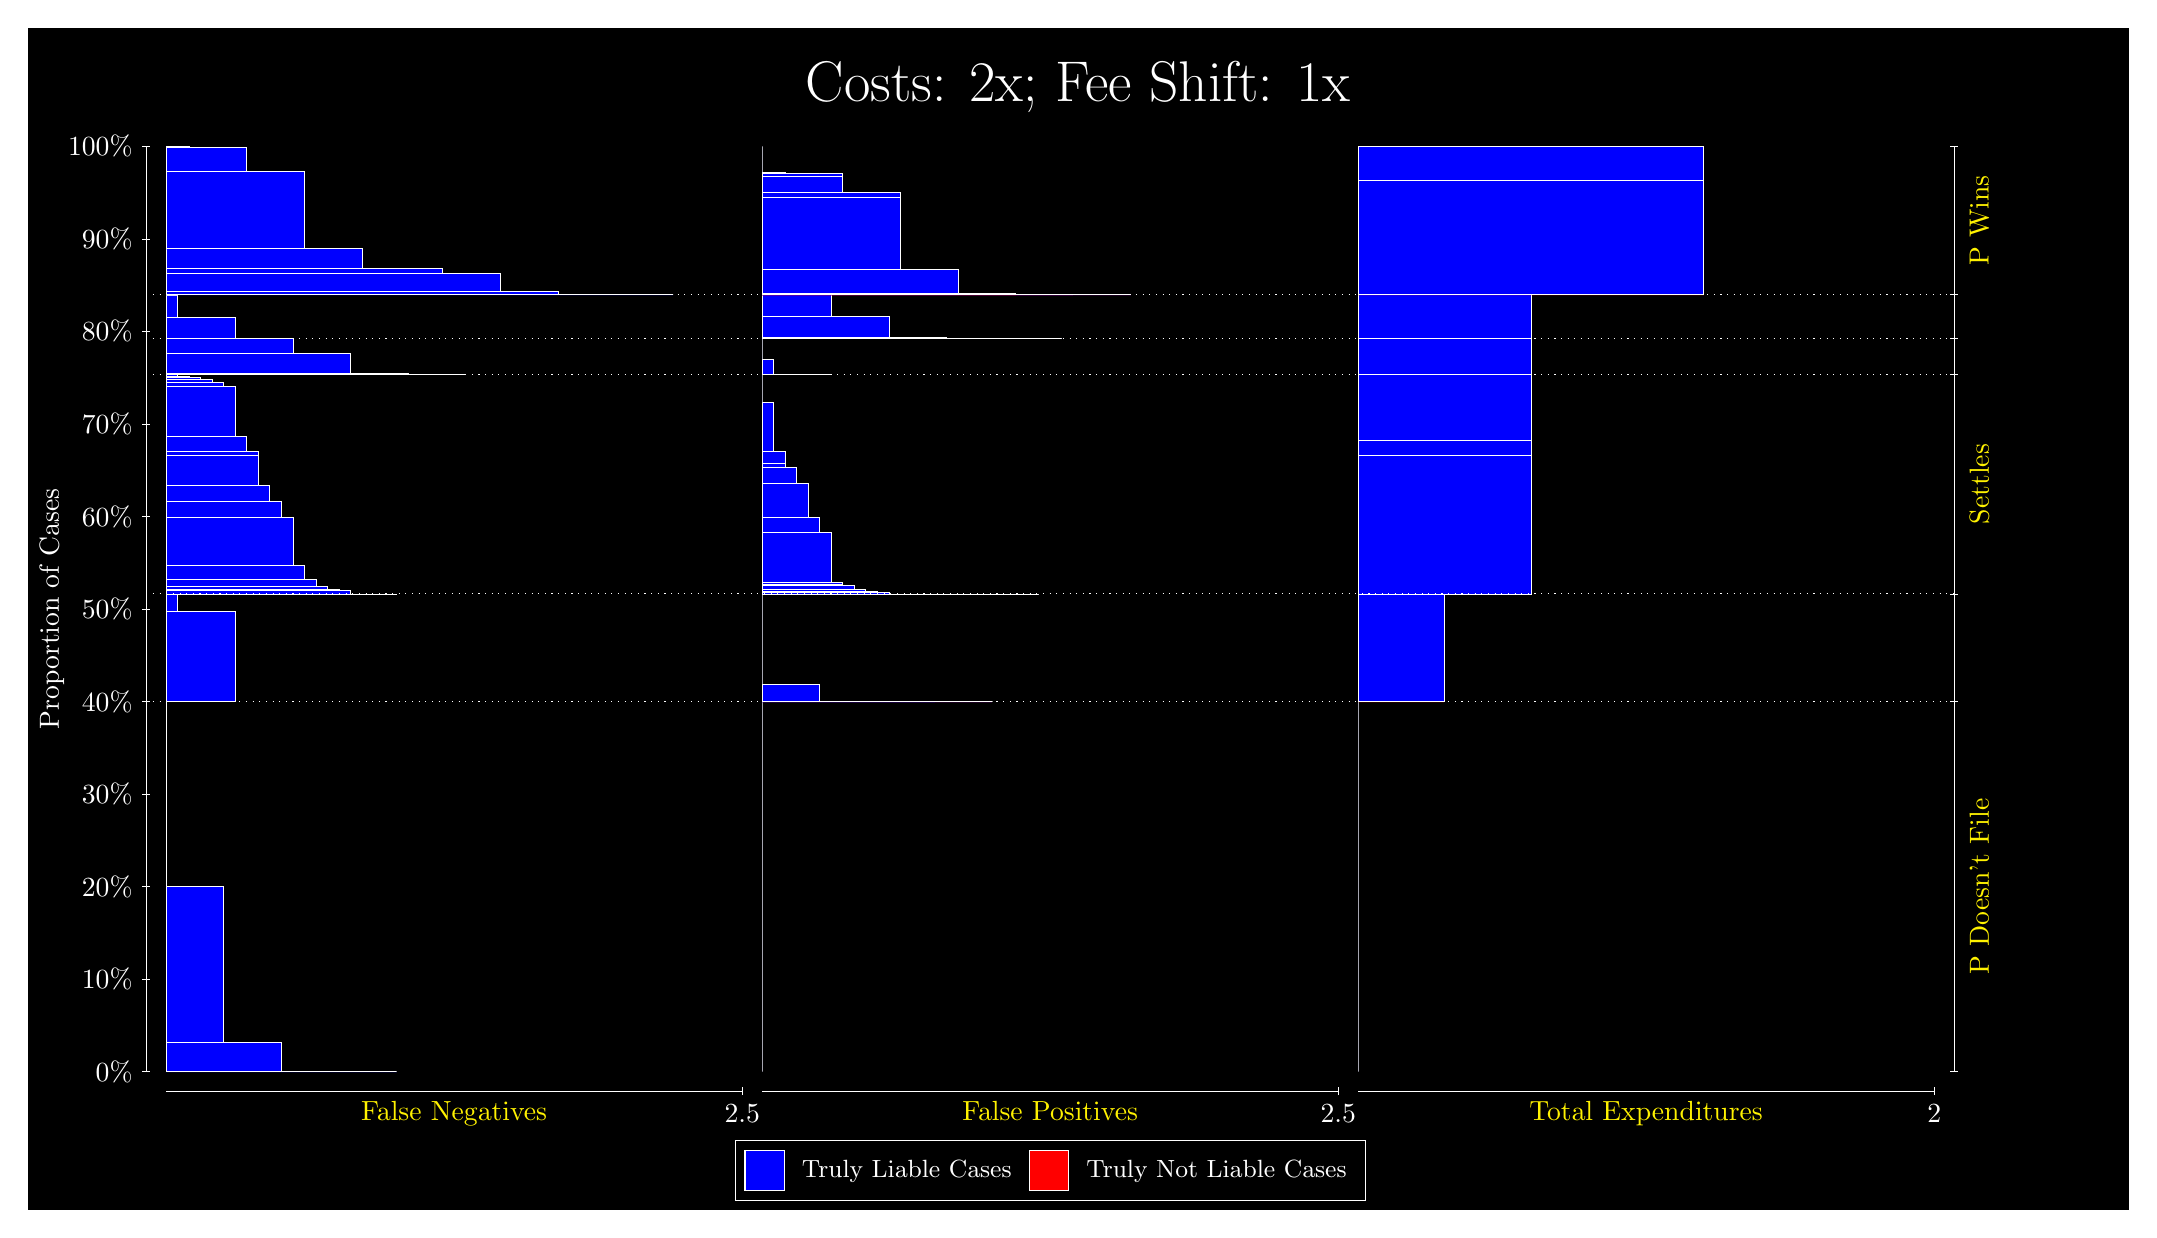
\begin{tikzpicture}
\draw[fill=black] (0,0) rectangle (26.667,15);
\draw[text=white] (0,13.5) rectangle (26.667,15) node[midway] {\huge Costs: 2x; Fee Shift: 1x};
\draw[white, very thin] (1.5,1.75) -- (1.5,13.5);
\node[rotate=90, text=white, anchor=center] at (0.3, 7.625) {Proportion of Cases};
\draw[white, very thin] (1.45,1.75) -- (1.55,1.75);
\node[text=white, anchor=east] at (1.45, 1.75) {0\%};
\draw[white, very thin] (1.45,2.925) -- (1.55,2.925);
\node[text=white, anchor=east] at (1.45, 2.925) {10\%};
\draw[white, very thin] (1.45,4.1) -- (1.55,4.1);
\node[text=white, anchor=east] at (1.45, 4.1) {20\%};
\draw[white, very thin] (1.45,5.275) -- (1.55,5.275);
\node[text=white, anchor=east] at (1.45, 5.275) {30\%};
\draw[white, very thin] (1.45,6.45) -- (1.55,6.45);
\node[text=white, anchor=east] at (1.45, 6.45) {40\%};
\draw[white, very thin] (1.45,7.625) -- (1.55,7.625);
\node[text=white, anchor=east] at (1.45, 7.625) {50\%};
\draw[white, very thin] (1.45,8.8) -- (1.55,8.8);
\node[text=white, anchor=east] at (1.45, 8.8) {60\%};
\draw[white, very thin] (1.45,9.975) -- (1.55,9.975);
\node[text=white, anchor=east] at (1.45, 9.975) {70\%};
\draw[white, very thin] (1.45,11.15) -- (1.55,11.15);
\node[text=white, anchor=east] at (1.45, 11.15) {80\%};
\draw[white, very thin] (1.45,12.325) -- (1.55,12.325);
\node[text=white, anchor=east] at (1.45, 12.325) {90\%};
\draw[white, very thin] (1.45,13.5) -- (1.55,13.5);
\node[text=white, anchor=east] at (1.45, 13.5) {100\%};

\draw[white, very thin] (24.457,1.75) -- (24.457,13.5);
\draw[white, very thin] (24.407,1.75) -- (24.507,1.75);
\node[anchor=west] at (24.407, 1.75) {};
\draw[white, very thin] (24.407,6.4489) -- (24.507,6.4489);
\node[anchor=west] at (24.407, 6.4489) {};
\draw[white, very thin] (24.407,7.8164) -- (24.507,7.8164);
\node[anchor=west] at (24.407, 7.8164) {};
\draw[white, very thin] (24.407,10.604) -- (24.507,10.604);
\node[anchor=west] at (24.407, 10.604) {};
\draw[white, very thin] (24.407,11.063) -- (24.507,11.063);
\node[anchor=west] at (24.407, 11.063) {};
\draw[white, very thin] (24.407,11.618) -- (24.507,11.618);
\node[anchor=west] at (24.407, 11.618) {};
\draw[white, very thin] (24.407,13.5) -- (24.507,13.5);
\node[anchor=west] at (24.407, 13.5) {};

\draw[white, very thin, fill=blue] (1.75,1.75) rectangle (4.6775,1.75);
\draw[white, very thin, fill=blue] (1.75,1.75) rectangle (3.9457,1.7532);
\draw[white, very thin, fill=blue] (1.75,1.7532) rectangle (3.2138,2.126);
\draw[white, very thin, fill=blue] (1.75,2.126) rectangle (2.4819,4.1027);
\draw[white, very thin, fill=red] (1.75,4.1027) rectangle (1.75,4.1027);
\draw[white, very thin, fill=blue] (1.75,4.1027) rectangle (1.75,6.4489);
\draw[white, very thin, fill=blue] (1.75,6.4489) rectangle (2.6283,7.593);
\draw[white, very thin, fill=blue] (1.75,7.593) rectangle (1.8964,7.8148);
\draw[white, very thin, fill=red] (1.75,7.8148) rectangle (1.75,7.8148);
\draw[white, very thin, fill=blue] (1.75,7.8148) rectangle (1.75,7.8164);
\draw[white, very thin, fill=blue] (1.75,7.8164) rectangle (4.6775,7.8165);
\draw[white, very thin, fill=blue] (1.75,7.8165) rectangle (4.3848,7.8168);
\draw[white, very thin, fill=blue] (1.75,7.8168) rectangle (4.092,7.8569);
\draw[white, very thin, fill=blue] (1.75,7.8569) rectangle (3.9457,7.8684);
\draw[white, very thin, fill=blue] (1.75,7.8684) rectangle (3.7993,7.9067);
\draw[white, very thin, fill=blue] (1.75,7.9067) rectangle (3.6529,7.9973);
\draw[white, very thin, fill=blue] (1.75,7.9973) rectangle (3.5065,8.174);
\draw[white, very thin, fill=blue] (1.75,8.174) rectangle (3.3602,8.7876);
\draw[white, very thin, fill=blue] (1.75,8.7876) rectangle (3.2138,8.9937);
\draw[white, very thin, fill=blue] (1.75,8.9937) rectangle (3.0674,9.1976);
\draw[white, very thin, fill=blue] (1.75,9.1976) rectangle (2.921,9.5712);
\draw[white, very thin, fill=blue] (1.75,9.5712) rectangle (2.921,9.6297);
\draw[white, very thin, fill=blue] (1.75,9.6297) rectangle (2.7746,9.8221);
\draw[white, very thin, fill=blue] (1.75,9.8221) rectangle (2.6283,10.457);
\draw[white, very thin, fill=blue] (1.75,10.457) rectangle (2.4819,10.5);
\draw[white, very thin, fill=blue] (1.75,10.5) rectangle (2.3355,10.547);
\draw[white, very thin, fill=blue] (1.75,10.547) rectangle (2.1891,10.563);
\draw[white, very thin, fill=blue] (1.75,10.563) rectangle (2.1891,10.571);
\draw[white, very thin, fill=blue] (1.75,10.571) rectangle (2.0428,10.581);
\draw[white, very thin, fill=blue] (1.75,10.581) rectangle (1.8964,10.603);
\draw[white, very thin, fill=red] (1.75,10.603) rectangle (1.75,10.603);
\draw[white, very thin, fill=blue] (1.75,10.603) rectangle (1.75,10.604);
\draw[white, very thin, fill=blue] (1.75,10.604) rectangle (5.5558,10.604);
\draw[white, very thin, fill=blue] (1.75,10.604) rectangle (4.8239,10.615);
\draw[white, very thin, fill=blue] (1.75,10.615) rectangle (4.092,10.876);
\draw[white, very thin, fill=blue] (1.75,10.876) rectangle (3.3602,11.06);
\draw[white, very thin, fill=blue] (1.75,11.06) rectangle (2.6283,11.063);
\draw[white, very thin, fill=red] (1.75,11.063) rectangle (1.75,11.063);
\draw[white, very thin, fill=blue] (1.75,11.063) rectangle (2.6283,11.335);
\draw[white, very thin, fill=blue] (1.75,11.335) rectangle (1.8964,11.602);
\draw[white, very thin, fill=red] (1.75,11.602) rectangle (1.75,11.602);
\draw[white, very thin, fill=blue] (1.75,11.602) rectangle (1.75,11.618);
\draw[white, very thin, fill=blue] (1.75,11.618) rectangle (8.1906,11.618);
\draw[white, very thin, fill=blue] (1.75,11.618) rectangle (7.4587,11.619);
\draw[white, very thin, fill=blue] (1.75,11.619) rectangle (6.7268,11.658);
\draw[white, very thin, fill=blue] (1.75,11.658) rectangle (5.9949,11.89);
\draw[white, very thin, fill=blue] (1.75,11.89) rectangle (5.7022,11.89);
\draw[white, very thin, fill=blue] (1.75,11.89) rectangle (5.2631,11.949);
\draw[white, very thin, fill=blue] (1.75,11.949) rectangle (4.9703,11.954);
\draw[white, very thin, fill=blue] (1.75,11.954) rectangle (4.5312,11.954);
\draw[white, very thin, fill=blue] (1.75,11.954) rectangle (4.2384,12.202);
\draw[white, very thin, fill=blue] (1.75,12.202) rectangle (3.7993,12.202);
\draw[white, very thin, fill=blue] (1.75,12.202) rectangle (3.5065,13.181);
\draw[white, very thin, fill=blue] (1.75,13.181) rectangle (2.7746,13.486);
\draw[white, very thin, fill=blue] (1.75,13.486) rectangle (2.0428,13.5);
\draw[white, very thin, fill=red] (1.75,13.5) rectangle (1.75,13.5);
\draw[white, very thin, fill=blue] (1.75,13.5) rectangle (1.75,13.5);
\draw[white, very thin, fill=red] (9.3189,1.75) rectangle (9.3189,1.75);
\draw[white, very thin, fill=blue] (9.3189,1.75) rectangle (9.3189,6.4489);
\draw[white, very thin, fill=red] (9.3189,6.4489) rectangle (12.246,6.4489);
\draw[white, very thin, fill=blue] (9.3189,6.4489) rectangle (12.246,6.4489);
\draw[white, very thin, fill=blue] (9.3189,6.4489) rectangle (11.515,6.4489);
\draw[white, very thin, fill=blue] (9.3189,6.4489) rectangle (10.783,6.4505);
\draw[white, very thin, fill=blue] (9.3189,6.4505) rectangle (10.051,6.6724);
\draw[white, very thin, fill=blue] (9.3189,6.6724) rectangle (9.3189,7.8164);
\draw[white, very thin, fill=red] (9.3189,7.8164) rectangle (12.832,7.8164);
\draw[white, very thin, fill=blue] (9.3189,7.8164) rectangle (12.832,7.8164);
\draw[white, very thin, fill=red] (9.3189,7.8164) rectangle (12.539,7.8164);
\draw[white, very thin, fill=blue] (9.3189,7.8164) rectangle (12.539,7.8164);
\draw[white, very thin, fill=red] (9.3189,7.8164) rectangle (12.246,7.8164);
\draw[white, very thin, fill=blue] (9.3189,7.8164) rectangle (12.246,7.8164);
\draw[white, very thin, fill=blue] (9.3189,7.8164) rectangle (12.1,7.8164);
\draw[white, very thin, fill=red] (9.3189,7.8164) rectangle (11.954,7.8164);
\draw[white, very thin, fill=blue] (9.3189,7.8164) rectangle (11.954,7.8164);
\draw[white, very thin, fill=blue] (9.3189,7.8164) rectangle (11.807,7.8164);
\draw[white, very thin, fill=red] (9.3189,7.8164) rectangle (11.661,7.8164);
\draw[white, very thin, fill=blue] (9.3189,7.8164) rectangle (11.661,7.8164);
\draw[white, very thin, fill=blue] (9.3189,7.8164) rectangle (11.515,7.8164);
\draw[white, very thin, fill=red] (9.3189,7.8164) rectangle (11.368,7.8164);
\draw[white, very thin, fill=blue] (9.3189,7.8164) rectangle (11.368,7.8165);
\draw[white, very thin, fill=blue] (9.3189,7.8165) rectangle (11.222,7.8166);
\draw[white, very thin, fill=blue] (9.3189,7.8166) rectangle (11.075,7.8172);
\draw[white, very thin, fill=red] (9.3189,7.8172) rectangle (11.075,7.8172);
\draw[white, very thin, fill=blue] (9.3189,7.8172) rectangle (11.075,7.8172);
\draw[white, very thin, fill=blue] (9.3189,7.8172) rectangle (10.929,7.8394);
\draw[white, very thin, fill=blue] (9.3189,7.8394) rectangle (10.783,7.8498);
\draw[white, very thin, fill=blue] (9.3189,7.8498) rectangle (10.636,7.8739);
\draw[white, very thin, fill=blue] (9.3189,7.8739) rectangle (10.49,7.9208);
\draw[white, very thin, fill=blue] (9.3189,7.9208) rectangle (10.344,7.9411);
\draw[white, very thin, fill=blue] (9.3189,7.9411) rectangle (10.344,7.9633);
\draw[white, very thin, fill=blue] (9.3189,7.9633) rectangle (10.197,8.5984);
\draw[white, very thin, fill=blue] (9.3189,8.5984) rectangle (10.051,8.7907);
\draw[white, very thin, fill=blue] (9.3189,8.7907) rectangle (9.9044,9.2229);
\draw[white, very thin, fill=blue] (9.3189,9.2229) rectangle (9.758,9.4267);
\draw[white, very thin, fill=blue] (9.3189,9.4267) rectangle (9.6116,9.4743);
\draw[white, very thin, fill=blue] (9.3189,9.4743) rectangle (9.6116,9.6328);
\draw[white, very thin, fill=blue] (9.3189,9.6328) rectangle (9.4652,10.246);
\draw[white, very thin, fill=blue] (9.3189,10.246) rectangle (9.3189,10.604);
\draw[white, very thin, fill=red] (9.3189,10.604) rectangle (10.197,10.604);
\draw[white, very thin, fill=blue] (9.3189,10.604) rectangle (10.197,10.606);
\draw[white, very thin, fill=blue] (9.3189,10.606) rectangle (9.4652,10.79);
\draw[white, very thin, fill=blue] (9.3189,10.79) rectangle (9.3189,11.063);
\draw[white, very thin, fill=red] (9.3189,11.063) rectangle (13.125,11.063);
\draw[white, very thin, fill=blue] (9.3189,11.063) rectangle (13.125,11.063);
\draw[white, very thin, fill=blue] (9.3189,11.063) rectangle (12.393,11.063);
\draw[white, very thin, fill=blue] (9.3189,11.063) rectangle (11.661,11.078);
\draw[white, very thin, fill=blue] (9.3189,11.078) rectangle (10.929,11.346);
\draw[white, very thin, fill=blue] (9.3189,11.346) rectangle (10.197,11.618);
\draw[white, very thin, fill=red] (9.3189,11.618) rectangle (14.003,11.618);
\draw[white, very thin, fill=blue] (9.3189,11.618) rectangle (14.003,11.618);
\draw[white, very thin, fill=red] (9.3189,11.618) rectangle (13.271,11.618);
\draw[white, very thin, fill=blue] (9.3189,11.618) rectangle (13.271,11.618);
\draw[white, very thin, fill=red] (9.3189,11.618) rectangle (12.539,11.618);
\draw[white, very thin, fill=blue] (9.3189,11.618) rectangle (12.539,11.632);
\draw[white, very thin, fill=blue] (9.3189,11.632) rectangle (11.807,11.937);
\draw[white, very thin, fill=red] (9.3189,11.937) rectangle (11.807,11.937);
\draw[white, very thin, fill=blue] (9.3189,11.937) rectangle (11.807,11.937);
\draw[white, very thin, fill=blue] (9.3189,11.937) rectangle (11.075,12.859);
\draw[white, very thin, fill=blue] (9.3189,12.859) rectangle (11.075,12.916);
\draw[white, very thin, fill=red] (9.3189,12.916) rectangle (10.783,12.916);
\draw[white, very thin, fill=blue] (9.3189,12.916) rectangle (10.783,12.916);
\draw[white, very thin, fill=blue] (9.3189,12.916) rectangle (10.344,13.125);
\draw[white, very thin, fill=blue] (9.3189,13.125) rectangle (10.344,13.164);
\draw[white, very thin, fill=red] (9.3189,13.164) rectangle (10.051,13.164);
\draw[white, very thin, fill=blue] (9.3189,13.164) rectangle (10.051,13.164);
\draw[white, very thin, fill=blue] (9.3189,13.164) rectangle (9.6116,13.169);
\draw[white, very thin, fill=blue] (9.3189,13.169) rectangle (9.6116,13.169);
\draw[white, very thin, fill=red] (9.3189,13.169) rectangle (9.3189,13.169);
\draw[white, very thin, fill=blue] (9.3189,13.169) rectangle (9.3189,13.5);
\draw[white, very thin, fill=red] (16.888,1.75) rectangle (16.888,1.75);
\draw[white, very thin, fill=blue] (16.888,1.75) rectangle (16.888,6.4489);
\draw[white, very thin, fill=red] (16.888,6.4489) rectangle (17.986,6.4489);
\draw[white, very thin, fill=blue] (16.888,6.4489) rectangle (17.986,7.8164);
\draw[white, very thin, fill=red] (16.888,7.8164) rectangle (19.083,7.8164);
\draw[white, very thin, fill=blue] (16.888,7.8164) rectangle (19.083,9.5753);
\draw[white, very thin, fill=red] (16.888,9.5753) rectangle (19.083,9.5753);
\draw[white, very thin, fill=blue] (16.888,9.5753) rectangle (19.083,9.7676);
\draw[white, very thin, fill=red] (16.888,9.7676) rectangle (19.083,9.7676);
\draw[white, very thin, fill=blue] (16.888,9.7676) rectangle (19.083,10.604);
\draw[white, very thin, fill=red] (16.888,10.604) rectangle (19.083,10.604);
\draw[white, very thin, fill=blue] (16.888,10.604) rectangle (19.083,11.063);
\draw[white, very thin, fill=red] (16.888,11.063) rectangle (19.083,11.063);
\draw[white, very thin, fill=blue] (16.888,11.063) rectangle (19.083,11.618);
\draw[white, very thin, fill=red] (16.888,11.618) rectangle (21.279,11.618);
\draw[white, very thin, fill=blue] (16.888,11.618) rectangle (21.279,13.073);
\draw[white, very thin, fill=red] (16.888,13.073) rectangle (21.279,13.073);
\draw[white, very thin, fill=blue] (16.888,13.073) rectangle (21.279,13.5);
\draw[white, dotted] (1.5,6.4489) -- (24.457,6.4489);
\draw[white, dotted] (1.5,7.8164) -- (24.457,7.8164);
\draw[white, dotted] (1.5,10.604) -- (24.457,10.604);
\draw[white, dotted] (1.5,11.063) -- (24.457,11.063);
\draw[white, dotted] (1.5,11.618) -- (24.457,11.618);
\draw[white, very thin] (1.75,1.5) -- (9.0689,1.5);
\node[text=yellow, anchor=north] at (5.4094, 1.5) {False Negatives};
\draw[white, very thin] (9.0689,1.45) -- (9.0689,1.55);
\node[text=white, anchor=north] at (9.0689, 1.45) {2.5};

\draw[white, very thin] (9.3189,1.5) -- (16.638,1.5);
\node[text=yellow, anchor=north] at (12.978, 1.5) {False Positives};
\draw[white, very thin] (16.638,1.45) -- (16.638,1.55);
\node[text=white, anchor=north] at (16.638, 1.45) {2.5};

\draw[white, very thin] (16.888,1.5) -- (24.207,1.5);
\node[text=yellow, anchor=north] at (20.547, 1.5) {Total Expenditures};
\draw[white, very thin] (24.207,1.45) -- (24.207,1.55);
\node[text=white, anchor=north] at (24.207, 1.45) {2};

\node[text=yellow, centered, rotate=90] at (24.777, 4.0995) {P Doesn't File};

\node[text=yellow, centered, rotate=90] at (24.777, 9.2102) {Settles};


\node[text=yellow, centered, rotate=90] at (24.777, 12.559) {P Wins};

\draw (12.978300999999998,1.5) node[draw=none] (baseCoordinate) {};
\begin{scope}[align=center]
        \matrix[scale=0.5, draw=white, below=0.5cm of baseCoordinate, nodes={draw}, column sep=0.1cm]{
            \node[rectangle, draw, minimum width=0.5cm, minimum height=0.5cm, fill=blue] {}; &
            \node[draw=none, font=\small, text=white] (B) {Truly Liable Cases}; &
            \node[rectangle, draw, minimum width=0.5cm, minimum height=0.5cm, fill=red] {}; &
            \node[draw=none, font=\small, text=white] (B) {Truly Not Liable Cases}; \\
            };
\end{scope}

\end{tikzpicture}
\end{document}